% ********** Testbeds Chapter **********
\chapter{Cryogenic Testbeds}
\label{cha:testbeds}
\epigraph{`Some people call it procrastination;\\I actually call it thinking.'}{\mbox{\textup{---\textsc{Hans Zimmer}}}}
%
\section{Introduction}\label{sec:testbeds_Introduction}
As is the case with all ultra-sensitive mid- to far-infrared detectors \parencite[as described by][]{Richards1994}, the silicon cold-electron bolometer requires cooling to extremely low temperatures in order to operate. This requirement can be seen from the description of cold-electron bolometers given in Chapter~\ref{cha:theory}. Since these detectors incorporate superconducting contacts to select only the most energetic (i.e. the hottest) electrons from the detector's absorber, it is important that the superconductor is cooled sufficiently that the superconducting energy gap is close to its maximum. For the detectors studied in this work, which used aluminium contacts, it was found  that cooling to approximately $\sim \nicefrac{T_{\mathrm{c}}\,}{4}$ ($300~\mathrm{mK}$) allowed the detector to operate reasonably. However, in order to arrive at as complete a study as possible, it was important to measure the electrical properties of the detectors to as low a temperature as possible.
\par 
To this end, several different cryogenic systems have been used in the course of this work. The most significant of these (those in which results presented in this thesis were taken) were a \gls{acr:He10} sorption refrigerator housed in a cryostat with a pulse tube cooler, and a \gls{acr:He7} sorption refrigerator mounted on the cold plate of a liquid helium cryostat.\footnote{Note: \gls{acr:He7} and \gls{acr:He10} here do not denote strange and exotic isotopes of helium but instead the combination of pumps which make up the soprtion refrigerator. Isotopes have been typeset with a leading superscript (i.e. \ce{^{4}He}). A \gls{acr:He7} refrigerator contains one \ce{^{4}He} pump and a \ce{^{3}He} pump, a \gls{acr:He10} refrigerator consists of a \gls{acr:He7} refrigerator used as a buffer stage for a second \ce{^{3}He} pump.} The reason for the use of these different systems was essentially due to availability and the associated costs of liquid helium. Primary measurements were carried out in the pulse-tube-cooled cryostat since this had lower running costs (due to not requiring a reservoir of liquid helium to be maintained). However (as will be seen later in this chapter), the system was not designed with the DC readout of sensitive detectors in mind and resulted in lower quality data than would have been desired; however, it did provide a useful facility for ascertaining whether or not a device was functional. The second system, which required the supply of liquid helium, contained optical windows, horns and filters to allow the detector to observe external sources. This chapter will cover the operational principles, along with the cryogenic performance and suitability for the required measurements of each of these systems.
%
\section{Sorption Refrigerators}\label{sec:sorptionRefrigerators}
Sorption refrigerators operate by the adsorption and desorption of a working gas (helium in the case of systems intended to operate at cryogenic temperatures) from a surface or other material (most commonly activated charcoal). The released gas flows through a pipe until it is cooled by a condensation point and liquified. This liquid is collected in a stage called the evaporator. The activated charcoal is then cooled, causing the gas evaporating from the liquid in the evaporator to become reattached to the charcoal, thus decreasing the pressure in the system and thus the temperature of the liquid in the evaporator. A simplified model of a single-stage sorption refrigerator is shown in Figure~\ref{fig:sorptionPumpCrossSec}.
\begin{figure}[tb]
\begin{center}
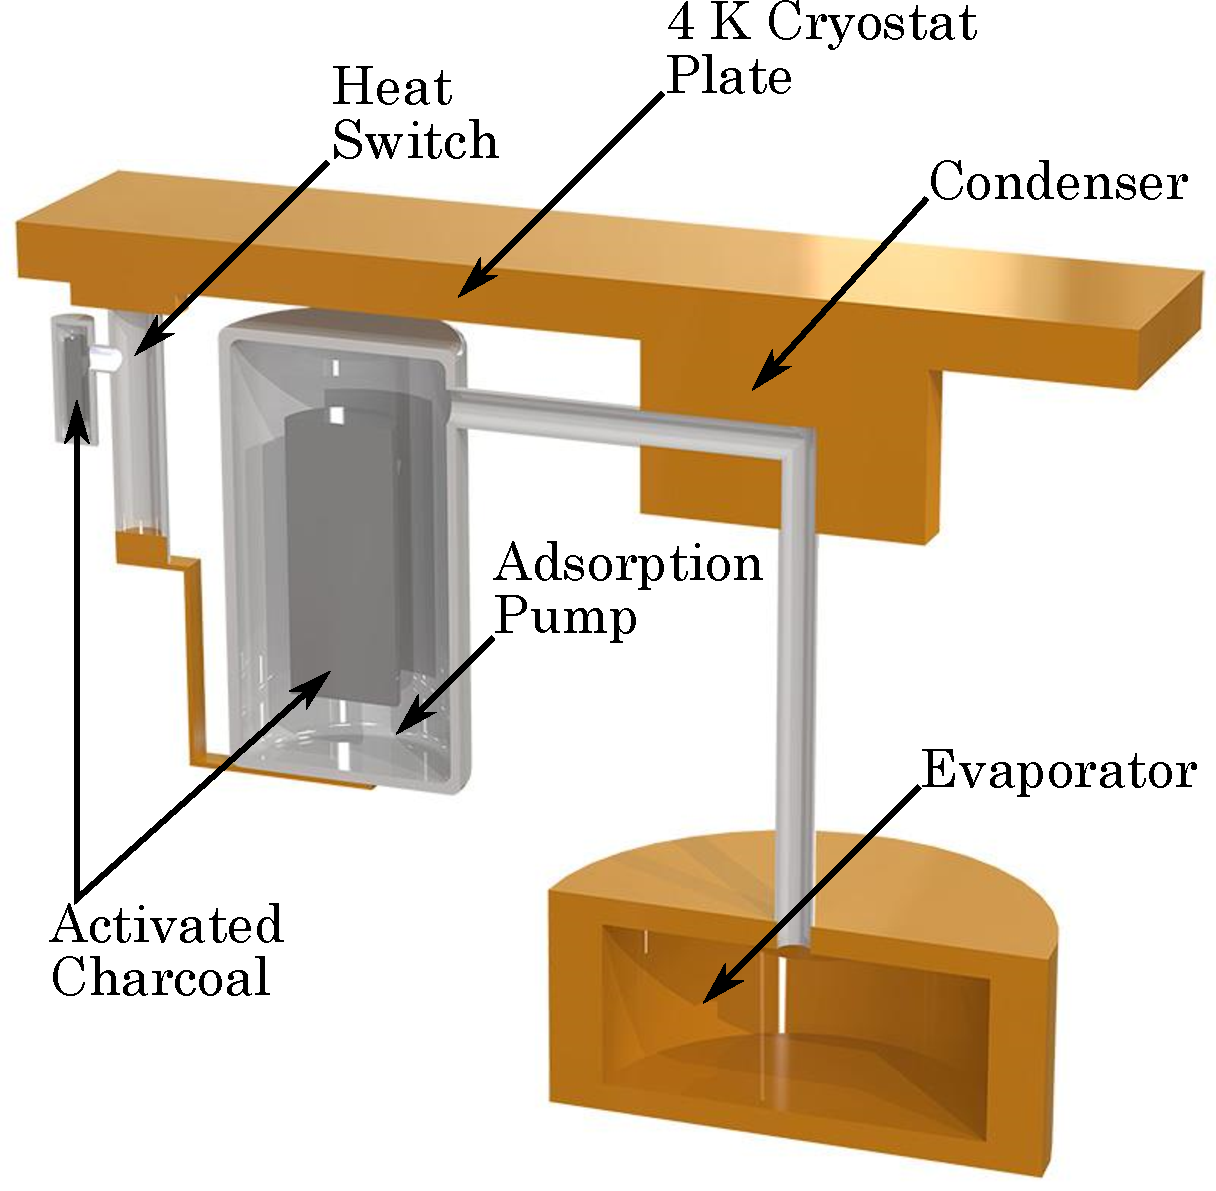
\includegraphics[width = 0.6\textwidth]{figures/sorptionPump}
\caption[Simplified model of the cross section of a sorption refrigerator]{Computer-generated model of the cross section of a sorption refrigerator. The 4-Kelvin plate of the cryostat is cooled by either a liquid-helium reservoir or a mechanical cooler (not shown in either case).}
\label{fig:sorptionPumpCrossSec}
\end{center}
\end{figure}
\par
Before the operation of such a refrigerator is discussed, it is useful to consider the working principles of gas-gap heat switches. Gas-gap heat switches are the most common type of heat switch used in conjuncture with sorption refrigerators. This can be thought of simply as a small sorption refrigerator. The heat switch is made of two copper caps connected by an extremely thin-walled stainless steel tube (which has negligible thermal conduction); attached to this, via a second thin tube, is a cylinder containing a charcoal getter. The heat switch also contains helium gas. When the switch is open (off), the helium is attached to the getter and there is little or no thermal conduction between the two copper caps. The heat switch is closed (switched on) by heating the charcoal, causing the helium to be released into the stainless steel tube, which results in the thermal conduction between the two copper caps increasing substantially.
\par
In order to understand a sorption refrigerator, it is perhaps easiest to consider the typical procedure followed to cycle such a system. The general procedure is as follows:
\begin{description}
\item[Cool system to working temperature.] In order to function, the condensing stage of the system must be cooled to the boiling point of the working gas (this is $4.2~\mathrm{K}$ for \ce{^{4}He}). This is performed by either: filling the cryostat in which the refrigerator is housed with liquid helium (in the case of \textit{wet} systems) or switching on the cryostat's mechanical cooler (for \textit{dry} systems) and waiting for all the parts of the system to thermalise.
\item[Heat the charcoal in the pump.] The pump is heated (usually via a film resistor mounted to the outside of the pump) causing the gas to be released from the activated charcoal (sometimes referred to as the \textit{getter}). As the charcoal is heated to above $10~\mathrm{K}$, helium will begin to be released and by $25~\mathrm{K}$ the vast majority will have been released.
\item[Helium condenses.] Increasing the temperature further causes the pressure within the refrigerator to increase, causing the gas to come into contact with the condenser, where it will condense. This liquid will then collect in the evaporator (situated beneath the condenser).
\item[Charcoal cooled.] The charcoal in the pump is then cooled again. This is performed using a heat switch. The heat switch has one side connected to the pump and the other to the cold plate of the cryostat. The closing of the heat switch creates a link between the pump and the cold plate of the cryostat and thus cools the pump.
\item[Pressure reduces.] As the charcoal in the pump cools to below $25~\mathrm{K}$, it is once again able to attract and hold gas. This means that as helium molecules evaporate from the liquid, they become attached to the activated charcoal (through adsorption) which causes the pressure in the system to reduce. This, in turn, lowers the temperature of the liquid in the evaporator along with the walls of the evaporator.
\end{description}
\par
The above process is for a single-stage helium-4 sorption refrigerator; such systems are capable of achieving temperatures of around $1~\mathrm{K}$ at the external walls of the evaporator. To achieve sub-Kelvin temperatures with a sorption refrigerator, one must use helium-3 as the working gas; this necessitates that the condensation point must be at a lower temperature (\ce{^{3}He} has a critical point of $3.3~\mathrm{K}$). 
\par 
In order to meet this requirement, it is common practice to use a helium-4 pump as a buffer stage to cool a condensation point on a helium-3 pump (this is what is referred to as a \gls{acr:He7} system).\footnote{It is worth mentioning that, as mechanical cooling technology (e.g. pulse tubes) is improving, these systems can, under low to medium thermal loads, offer sufficiently low temperatures to cycle a helium-3 sorption cooler directly, without the need of a buffer stage.} This technique was first reported by \textcite{DallOglio1991} who, at the time, achieved a minimum temperature of $300~\mathrm{mK}$ at the evaporator of the \ce{^{3}He} pump.
\par 
Further cooling can be achieved with sorption refrigerators by using the \gls{acr:He7} system described above to a cool a further helium-3 pump (thus making a \gls{acr:He10} system). This type of system was first introduced by \textcite{Bhatia2000} who described a system capable of achieving a minimum temperature of $234~\mathrm{mK}$ for 20 hours under minimal thermal loading ($\approx 0.9~\mathrm{\upmu W}$) or $242~\mathrm{mK}$ for 12 hours under a total thermal load of $3.9~\mathrm{\upmu W}$. Further improvements to the design of such systems, coupled with the lower starting temperatures offered by pulse tube coolers, has resulted in minimum operating temperatures of lower than $220~\mathrm{mK}$ being achieved under realistic experimental thermal loading.
%
\section{Systems Used in This Work}\label{sec:cryostats}
Two systems have been used for the majority of the low-temperature measurements presented in this work. These were: a cryostat with a pulse-tube cooler upon which a \gls{acr:He10} sorption refrigerator was mounted; and a liquid-helium cryostat, containing  windows to facilitate optical measurements, in which a \gls{acr:He7} sorption refrigerator was mounted. Each of these systems served a specific role, such as: facilitating optical measurement of detectors or characterisation at extremely low temperatures. These systems are discussed in greater detail in the following subsections.
%
\subsection{Pulse-Tube-Cooled Cryostat with He10 Sorption Refrigerator}
\label{ssec:Aloysius}
The first system used to characterise silicon cold-electron bolometers was a pulse-tube-cooled cryostat incorporating a \gls{acr:He10} sorption refrigerator. This system had a large cold plate ($260~\mathrm{mm}$ in diameter), which could be cooled to a minimum temperature of $220~\mathrm{mK}$, which could be maintained for more than 48 hours. The system also contained a set of windows to enable the measurement of a detector's response to an external source. These windows were not used for the most part, however, since an alternative system (discussed later in this section) enabled a much more complete optical study of a detector.
\par 
This cryostat was mainly used for measurements such as the initial verification of the device's function (i.e. whether tunnelling contacts to the silicon absorber had formed correctly), along with dark characterisation of the device (i.e. measuring the current-voltage relationship of the detector at various bath temperatures). It is worth mentioning that pulse tube cooler based cryogenic systems can contribute  additional, undesired, components when measuring noise spectra. These are caused by the pulsing of the mechanical cooler introducing movement at various stages of the cryostat. This movement can cause any of the following: thermal oscillations, movement of wiring (causing electrical variations through either changes to the wiring's capacitance or through induction), or alternations to the optical alignment of components. Clearly, in order to accurately measure the performance of any device mounted within such a system, it is vital not only to discover the magnitude of these effects but also to reduce their presence as much as possible. The various effects of microphonics, along with a considerably more detailed explanation of their introduction, is given by \textcite{Bhatia1999}. In order to reduce the effect of these microphonics, some form of dampening is required to reduce the force exerted on the various stages of the cryostat.
\begin{figure}[tb]
\begin{center}
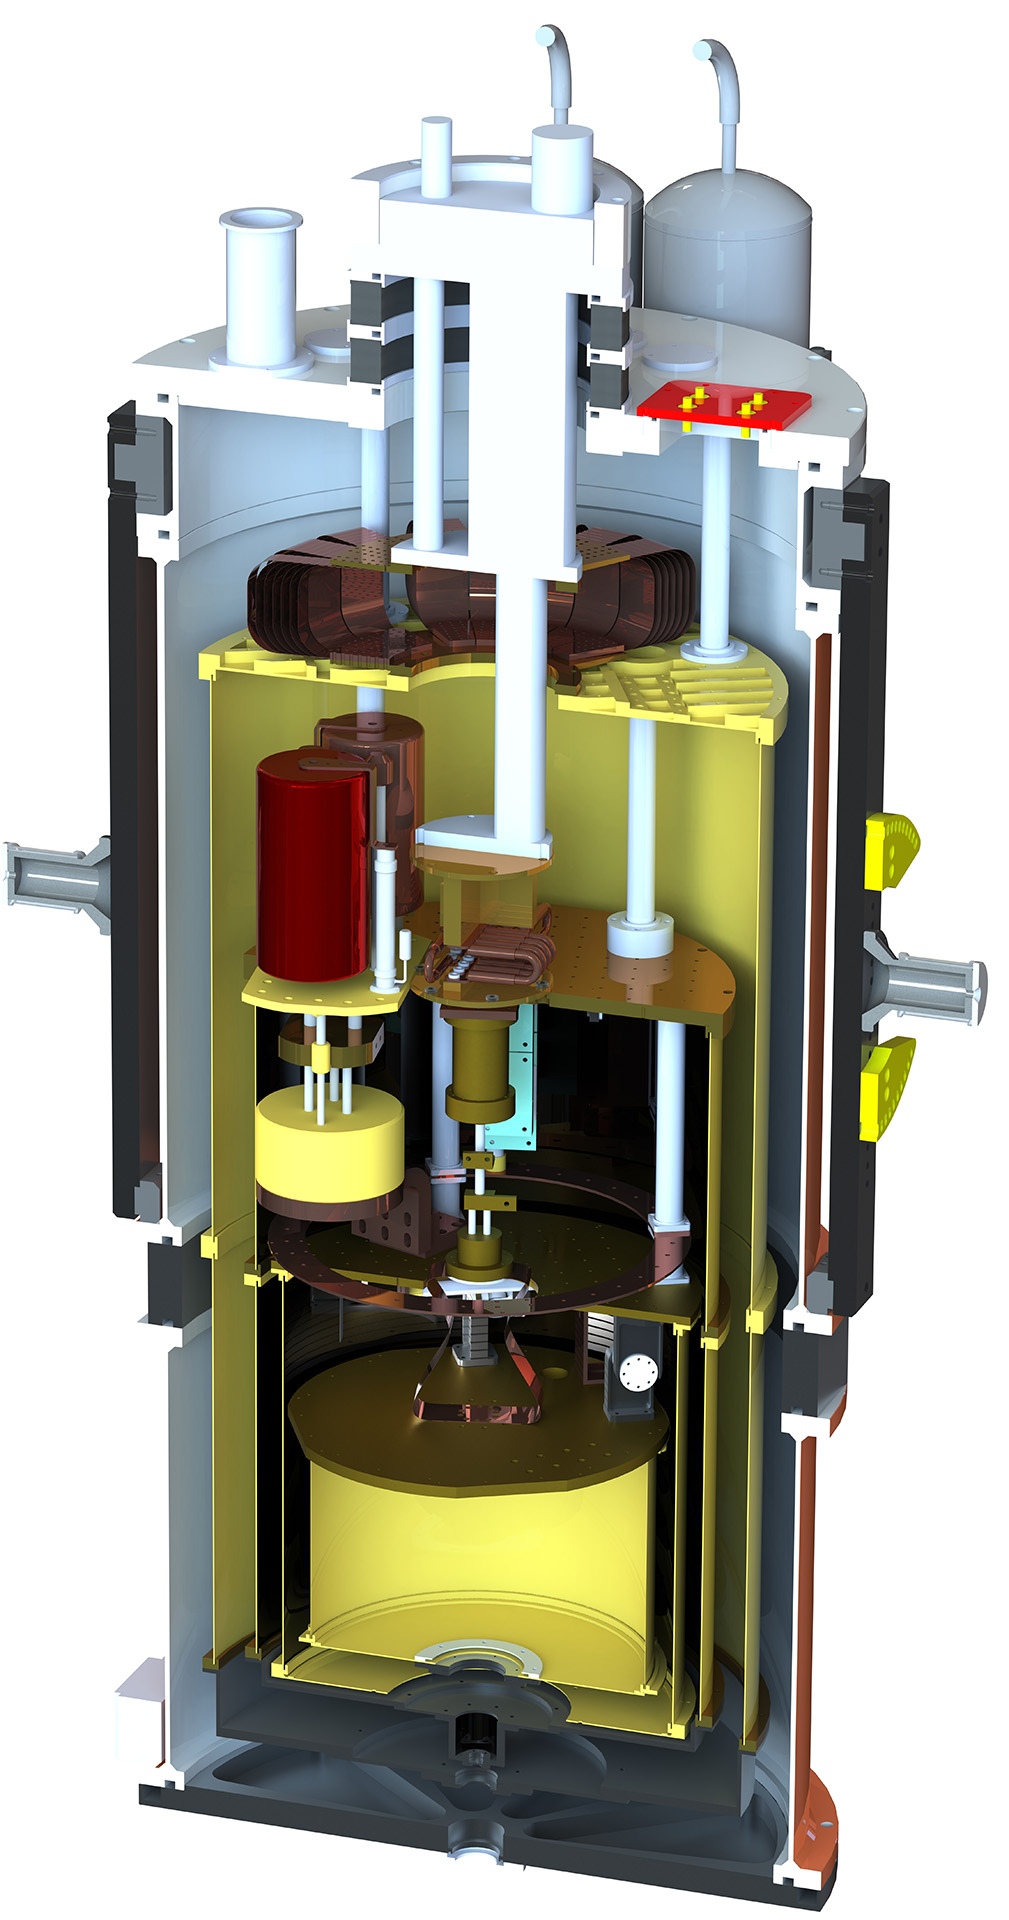
\includegraphics[height = 0.5\textheight]{figures/Aloysius1920}
\caption[Computer-generated model of the pulse-tube cooled cryostat]{Computer-generated model of pulse-tube cooled cryostat. Along with the various sorption pumps and heat switches, the damping stages can also be seen; these are (from top to bottom) the (black) rubber rings via which the pulse tube system is mounted to the cryostat, the bent copper-shim springs, the copper braid connecting the $65~\mathrm{K}$ stage of the pulse tube cooler the plate and copper shim connecting the condenser of the second \ce{^{3}He} sorption pump to the final cold plate.}
\label{fig:Aloysius}
\end{center}
\end{figure}
\begin{figure}[tb]
\begin{center}
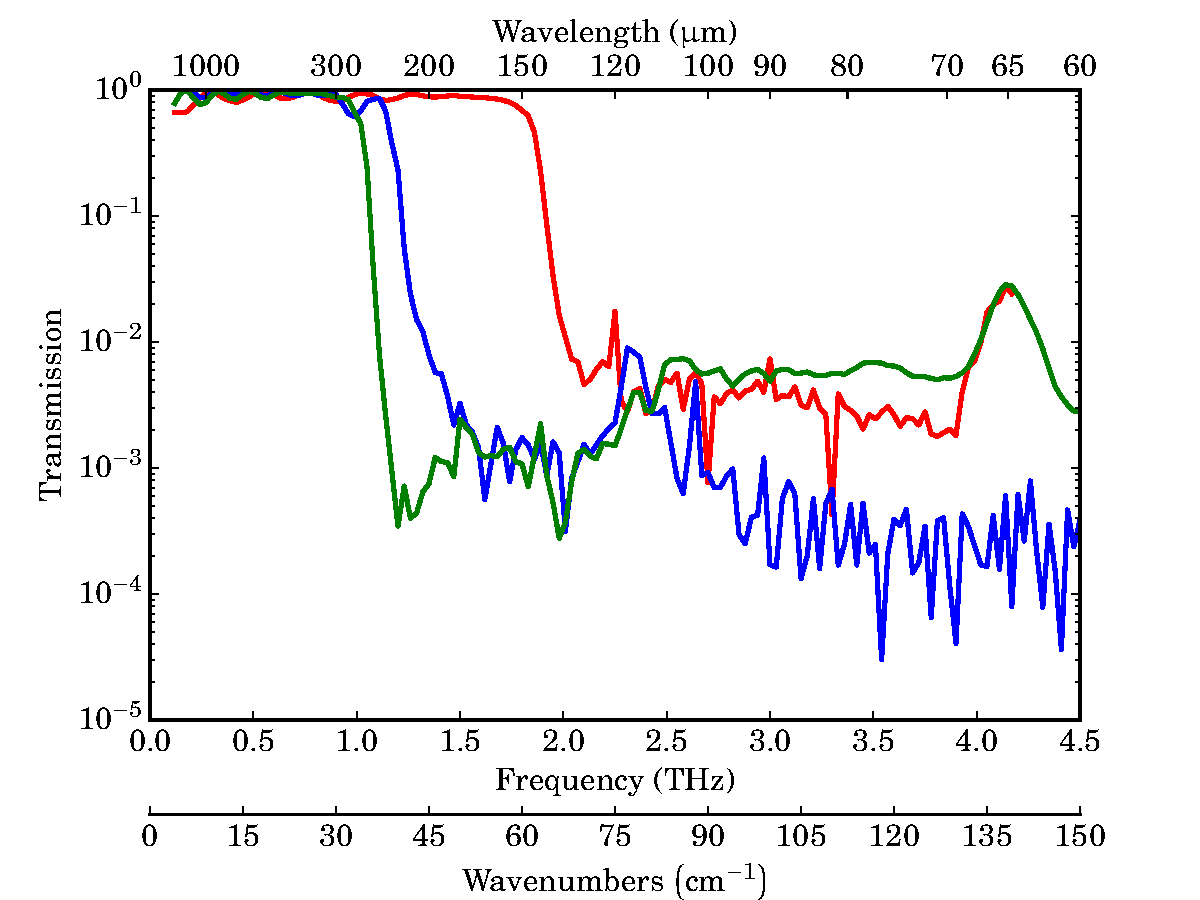
\includegraphics[width = 1.0\textwidth]{figures/AloysiusFilters}
\caption[Filters used for optical measurement in the pulse-tube cooled cryostat]{Filters mounted at various stages of the pulse-tube cooled cryostat for optical measurements. Red---$60~\mathrm{cm}^{-1}$ low-pass edge filter, mounted on the 60-K shield; blue---$43~\mathrm{cm}^{-1}$ low-pass edge, mounted on the 4-K shield; green---$33~\mathrm{cm}^{-1}$ low-pass edge, mounted on the 350-mK shield.}
\label{fig:AloysiusFilters}
\end{center}
\end{figure}
\par 
In the case of this system, microphonics have been reduced by the deployment of four damping stages. Firstly, the pulse tube cooler's motor is electrically decoupled from the cryostat itself; this is performed by sitting the motor on a layer of plastic and by adding \gls{acr:PTFE} spacers to the lines between the motor and the pulse tube head; on the outside of the cryostat, instead of mounting the pulse tube cooler head directly to the outer vacuum-can, a number of rubber spacer rings (shore hardness 40) are placed between the cryostat and the head, these are sufficiently clamped to ensure a hermetic seal but allow a degree of movement to absorb some of the vibrational energy. Secondly, at the first stage of the pulse tube cooler (nominally at $65~\mathrm{K}$), the pulse tube cooler is connected to the cold plate via multiple pieces of thin copper shim bent into a c-shape; these act like springs, dampening any vibration, while still creating a good thermal link between the pulse tube cooler and the plate. At the second stage of the pulse tube cooler (nominally $3\mbox{--}4.2~\mathrm{K}$), a similar technique is used whereby the pulse tube cooler and the cold plate are connected via multiple strands of copper braid; this again affords a good thermal link while damping vibrations. Finally, the coldest stage of the system (that cooled by the second \ce{^{3}He} pump of the He10 sorption cooler) is connected to the pump via more copper shim (similar to that described earlier). All the cold plates of the system, with the exception of the coldest stage, are connected to the cryostat's outter vacuum shield by hollow stainless-steel supports with thin (compared to their length) walls. The coldest stage uses rigid supports containing sapphire-sapphire contacts \parencite[these have been described by][]{Bintley2007}. A computer-generated model of this system, showing these features along with various other components can be seen in Figure~\ref{fig:Aloysius}.
\par 
For optical measurements in this system, a set of metal-mesh filters \parencite[as described by][]{Ade2006} were used. These not only reduced the thermal load on the colder stages of the cryostat (those with the least cooling power) but also reduced the out-of-band power on the detector (i.e. radiation with frequencies not of interest for the study being carried out). The transmission profiles of these filters can be seen in Figure~\ref{fig:AloysiusFilters}. An additional band-pass filter with 3-dB bandwidth of $50~\mathrm{GHz}$ centred around $150~\mathrm{GHz}$ was also used. This was mounted on the front of the detector holder and is not shown in Figure~\ref{fig:AloysiusFilters}.
%
\subsection{Liquid Helium Cryostat with He7 Sorption Refrigerator}
\label{ssec:CookieMonster}
The second system used to characterise detectors was a second liquid helium cryostat, this time with a \gls{acr:He7} sorption refrigerator. This system was used for the vast majority of optical measurements taken, including measuring the spectral response of the detector. This system was well suited to such measurements, due to the inclusion a set of back-to-back horns, which produced a well defined beam of radiation at the detector stage.
\begin{figure}[tb]
\begin{center}
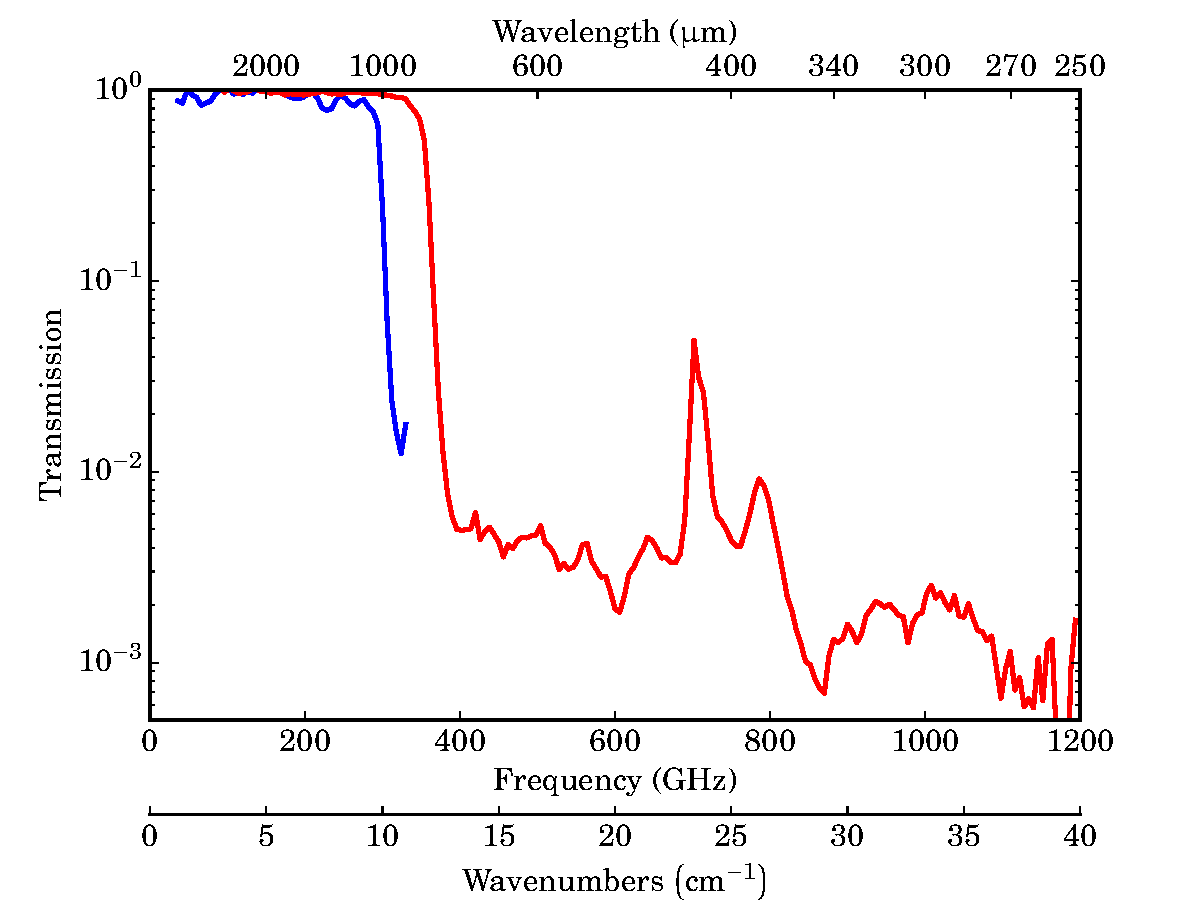
\includegraphics[width = 1.0\textwidth]{figures/CookieMonsterFilters}
\caption[Filter profile of filters used in the optical measurement cryostat]{Filter profile of filters used in optical measurement cryostat. Red---$12~\mathrm{cm}^{-1}$ low-pass edge filter mounted on the back-to-back horns at $4.2~\mathrm{K}$; blue---$10~\mathrm{cm}^{-1}$ low-pass edge filter mounted on the device holder at $350~\mathrm{mK}$. A set of thermal blockers were also used to reduce the power load on the cold stage of the cryostat; these were close to $100~\%$ transparent at the frequencies shown and, as such, have not been included.}
\label{fig:CookieMonsterFilters}
\end{center}
\end{figure}
\par 
As was the case with the pulse-tube cooled system, a number of filters were used to remove the out-of-band radiation, these are shown in Figure~\ref{fig:CookieMonsterFilters}. The vacuum jacket of the cryostat contained a large ($90~\mathrm{mm}$) \gls{acr:UHMWPE} window. This blocked the visible and near-infrared light, as well as ensuring that the vacuum was maintained. The 77-K and 4-K shields contained thermal-blocking filters; these are close to $100~\%$ transparent in the frequency range shown in Figure~\ref{fig:CookieMonsterFilters} and, as such, the profiles of these have not been plotted. In front of the back-to-back horns (at $4.2~\mathrm{K}$ but after the thermal blocker), a $12~\mathrm{cm}^{-1}$ low-pass edge filter was used (this is the red line in Figure~\ref{fig:CookieMonsterFilters}). The device holder, which was mounted on the $350~\mathrm{mK}$ stage of the cryostat, was fitted with a $10~\mathrm{cm}^{-1}$ low-pass edge filter. No bandpass filters were used to further reduce the spectral range of the incident radiation, since this would obviously prohibit any meaningful study of a detector's spectral response.
\begin{figure}[tb]
\begin{center}
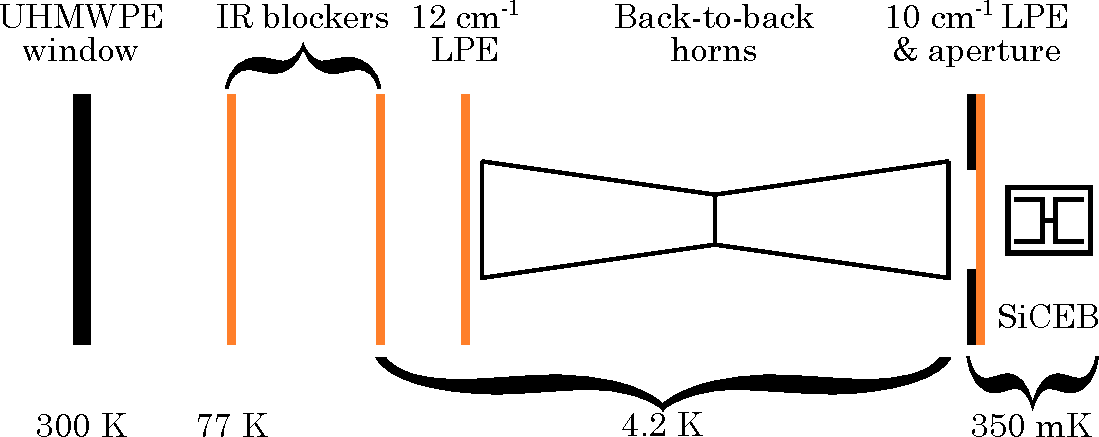
\includegraphics[width = 0.8\textwidth]{figures/CookieMonsterOptics}
\caption[Optical components housed in cryostat used for optical measurements]{Optical components housed in cryostat used for optical measurements.\glsadd{acr:UHMWPE}\glsadd{acr:IR}\glsadd{acr:LPE}}
\label{fig:CookieMonsterOptics}
\end{center}
\end{figure}
\par
The key optical components in this system were a pair of back-to-back corrugated horns, these were mounted at $4.2~\mathrm{mK}$ in a shield surrounding the 350-mK detector stage. These back-to-back horns produced an excellent Gaussian beam with low side-lobes. This horn arrangement is very similar to that used on \textit{Planck}'s \gls{acr:HFI} instrument as described by \textcite{Maffei2010}. A simplistic schematic of the optical configuration of this cryostat is shown in Figure~\ref{fig:CookieMonsterOptics}. A photograph of this system, in which the outer \gls{acr:UHMWPE} window can be seen, is shown in Figure~\ref{fig:CookieMonster}. 
\begin{figure}[tb]
\begin{center}
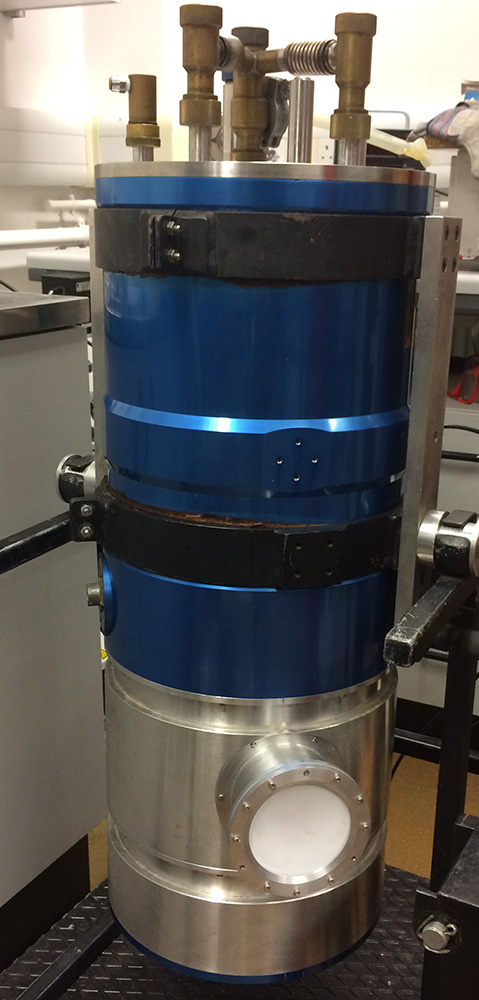
\includegraphics[height = 0.5\textheight]{figures/CookieMonster}
\caption[Photograph of cryostat used for optical measurements]{Photograph of cryostat used for optical measurements. The relatively large \gls{acr:UHMWPE} window can be seen towards the bottom of the photograph.}
\label{fig:CookieMonster}
\end{center}
\end{figure}

%
\section{Detector Holder}\label{sec:detectorHolder}
In order for the detectors to be characterised, they needed to be mounted in a holder which not only held them firmly in place, but also facilitated easy electrical connections, along with ensuring that only desired radiation was incident on the detector. Such a holder was manufactured in-house by a computer-numerical-control mill. The holder (shown in Figure~\ref{fig:deviceHolder}) included an aperture through which light could enter the holder for optical testing; a metal-mesh filter was clamped behind the aperture. For dark measurement, the filter could be replaced by a blank.
\par 
The various components of the holder all included lipped edges, which ensured that the holder was reasonably light-tight. A \gls{acr:PTFE} ring was used to clamp the silicon lens in place, this ring also ensured the lens was correctly aligned. A \glsfirst{acr:PCB}, wired to a micro-miniature D-type connector, allowed for simple connection to the detector holder. The electrical connection from the connector to the detector itself was completed by aluminium wire bonds between the printed circuit board and the detector.\footnote{The circuit board was gold plated to make the wire bonds more reliable.} The detector was secured in the holder via careful glueing, with GE varnish, to a piece of silicon (matched to the lens), which, in turn, was glued to the rear of the circuit board. When glueing the detector to this silicon, it was important to ensure that the GE varnish was only present at the edges and did not seep under the detector chip, since this would interfere with the radiation incident on the detector (which was rear-illuminated through the silicon substrate). A computer-generated model of the device holder can be seen in Figures~\ref{fig:detectorHolder_exploded} and \ref{fig:detectorHolder_cross}, which show an exploded view of the various components of the holder (including the detector chip itself) and a cross-section of the fully assembled holder.
\begin{figure}[tb]
\begin{center}
\subfloat[]{
	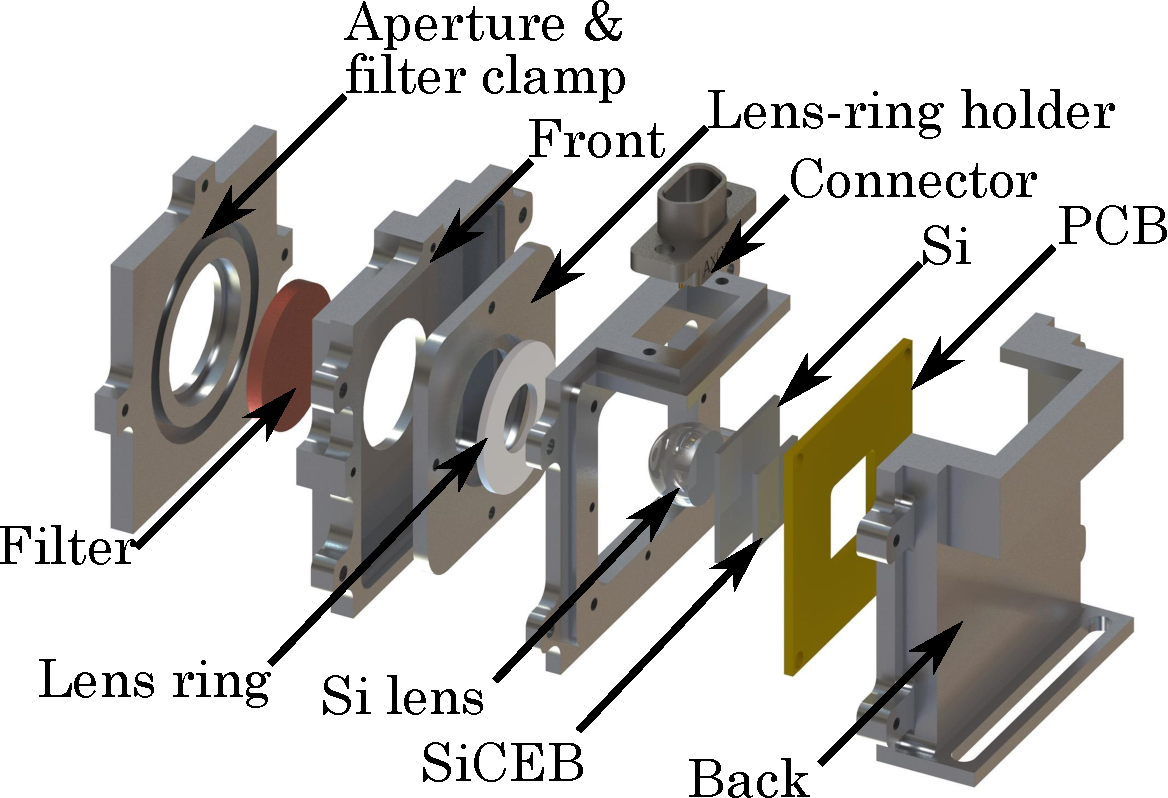
\includegraphics[width=0.6\textwidth]{figures/deviceHolder_exploded}
	\label{fig:detectorHolder_exploded}
}\\
\subfloat[]{
	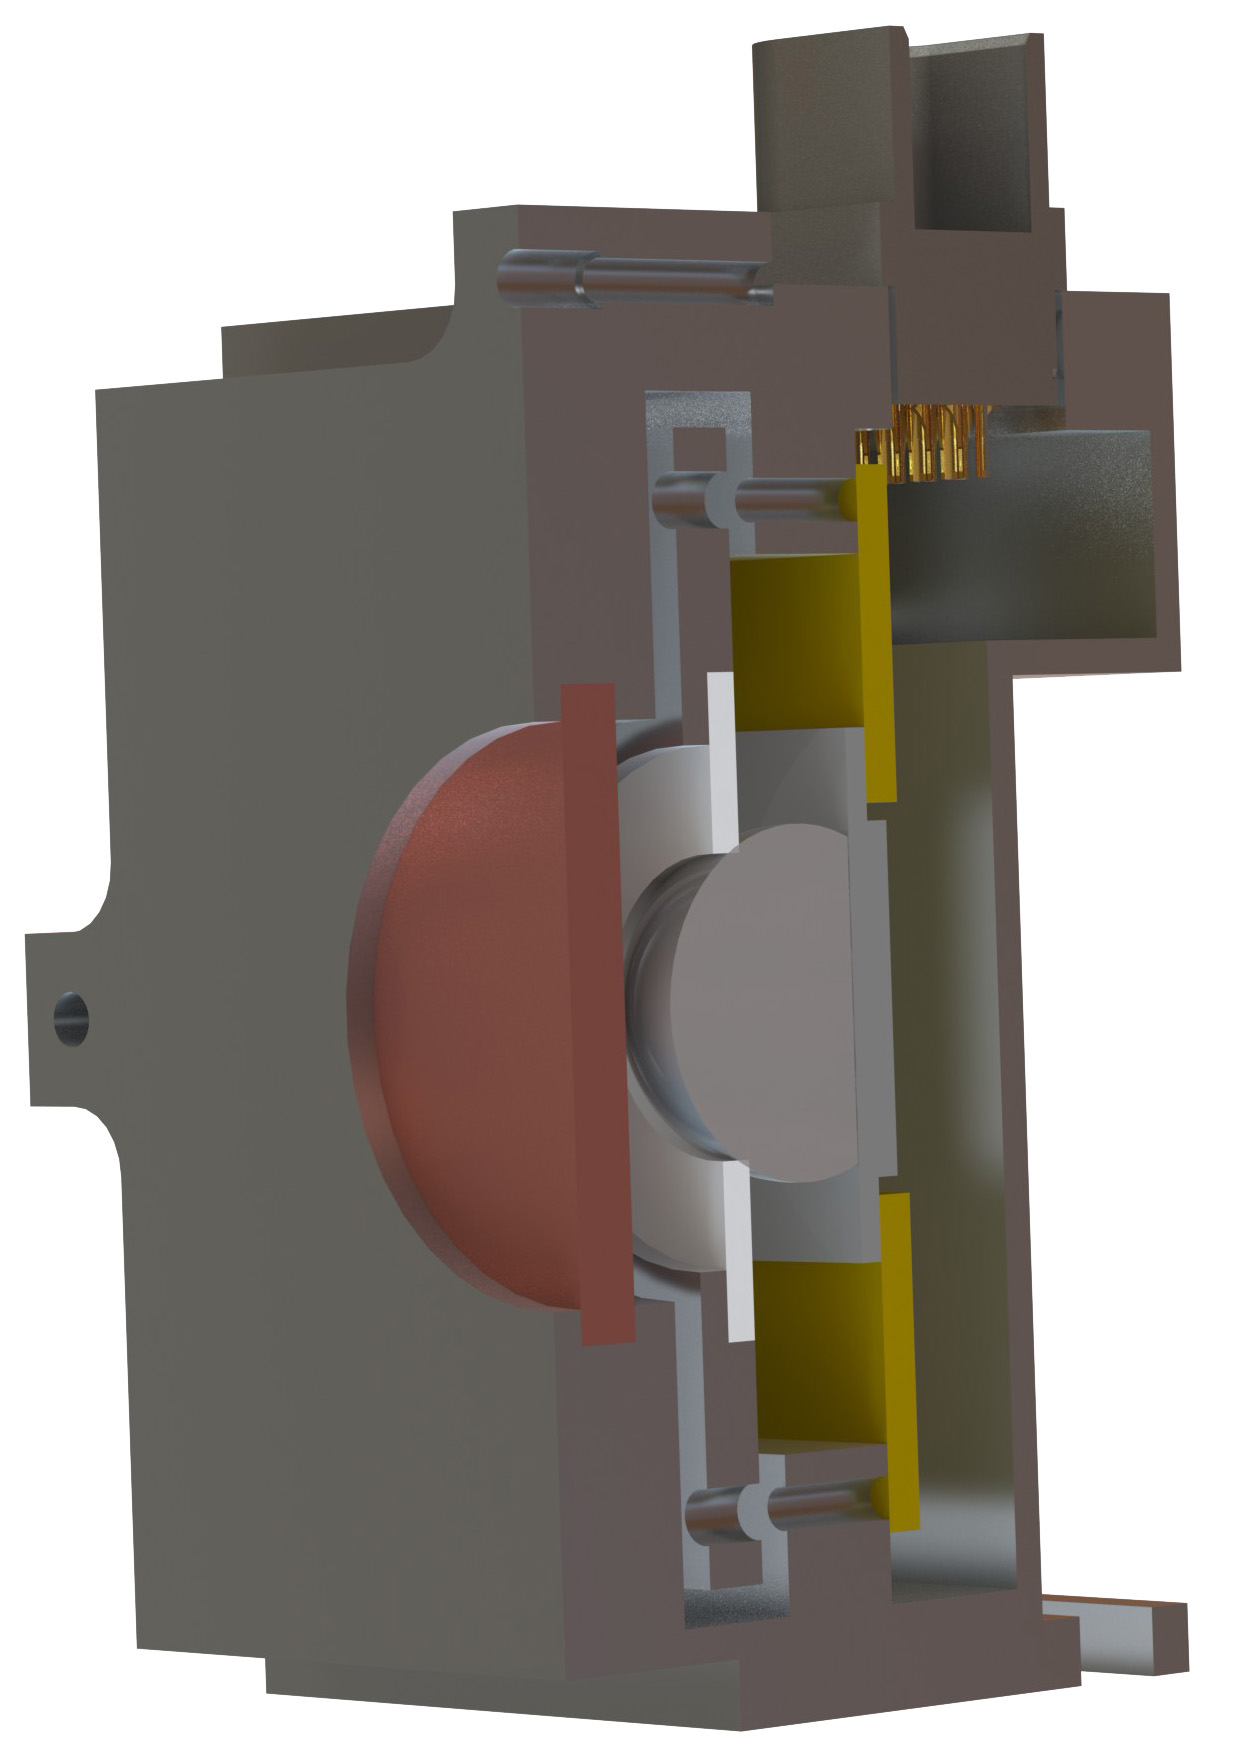
\includegraphics[width=0.3\textwidth]{figures/deviceHolder}
	\label{fig:detectorHolder_cross}
}
\caption[Detector holder]{Computer-generated model of the detector holder. (a) Exploded view of the detector holder, showing the various components; (b) cross-sectional view of the assembled detector holder.\glsadd{acr:PCB}}
\label{fig:deviceHolder}
\end{center}
\end{figure}
\par 
At cryogenic temperatures, assemblies of mechanical components, such as the device holder described here, it is vital to pay close attention to how the various components expand or contract relative to each other as they are cooled. The vast majority of the device holder used here was created from machined aluminium and thus the aluminium-aluminium interfaces were not of concern. However, particular attention was needed regarding the silicon lens and its \gls{acr:PTFE} securing ring. While the ring was clamped firmly to the lens and thin enough that it was capable of deflection while maintaining a firm contact to the lens, it is possible that as the two components were cooled, the ring may become loose and the lens might move. In order to explore this, we examined the coefficients of expansion, $\alpha$, for the two materials, defined as:
\begin{align}
\alpha = \frac{1}{x}\frac{\d x}{\d T}\,, \label{eqn:CTE}
\end{align}
where $x$ is the length of the material and $T$ is the temperature. Values for $\alpha$ are given in many standard reference tables and usually stated for a final temperature. \textcite{Kaye1995} states that for silicon cooled from room temperature (taken to be $293~\mathrm{K}$) to $100~\mathrm{K}$ is $-0.4\times 10^{-6}~\mathrm{K^{-1}}$; at the point of clamping the lens diameter was $8.5~\mathrm{mm}$, so by the use of Equation~\ref{eqn:CTE} we find that by cooling over this range the lens expands by:
\begin{align}
\Delta x &= 8.5\times 10^{-3} \times -0.4\times 10^{-6} 
	\times \left(100 - 293\right)\, \nonumber \\
	&= 0.65~\mathrm{\upmu m}\,.
\end{align}
That is to say the lens expands by less than one micrometre at the interface with the clamp. \textcite{NBS1961} gives a value of $\alpha = 21.1 \times 10^{-3}~\mathrm{K^{-1}}$ for \gls{acr:PTFE} when cooled from room temperature to $20~\mathrm{K}$; note this is a greater range than is given for silicon by \textcite{Kaye1995}, however it serves as a good indication all the same. By again using Equation~\ref{eqn:CTE}, we find that when cooled to $20~\mathrm{K}$, the silicon ring expands by:
\begin{align}
\Delta x &= 8.5 \times 10^{-3} \times 21.1\times 10^{-3}
	\times \left(20 - 293\right)\, \nonumber \\
	&=-49~\mathrm{\upmu m}\,.
\end{align} 
Meaning that the \gls{acr:PTFE} ring is shrinking by nearly $50~\mathrm{\upmu m}$. The \gls{acr:PTFE} ring is not mechanically fixed or glued to any other surface and thus is free to contract about its centre. This analysis shows that, when cooled, the lens marginally expands while the clamping ring contracts and so we deduce that at lower temperatures the lens should be clamped to the detector firmly. This justifies the choice of materials here and removes any concerns that the lens may become loose under thermal cycling. it is worth noting that the small values for the relative expansion and contraction discussed here could also be accommodated by ensuring the \gls{acr:PTFE} ring was slightly deflected when clamping the lens.
